% --------------------------------------------------------------------------- %
% Poster for the 5th ACM International Symposium on Pervasive Displays        %
% Oulu, Finland                                                               %
% 20-22 June, 2016                                                            %
% --------------------------------------------------------------------------- %
%
% Poster template reference
% http://www.brian-amberg.de/uni/poster/
%
% --------------------------------------------------------------------------- %


\documentclass[a0paper,portrait]{baposter}

\usepackage{calc}
\usepackage{graphicx}
\usepackage{amsmath}
\usepackage{amssymb}
\usepackage{relsize}
\usepackage{multirow}
\usepackage{rotating}
\usepackage{bm}
\usepackage{url}

\usepackage{graphicx}
\usepackage{multicol}

\newcommand{\captionfont}{\footnotesize}

\graphicspath{{images/}{../images/}}
\usetikzlibrary{calc}

\newcommand{\SET}[1]  {\ensuremath{\mathcal{#1}}}
\newcommand{\MAT}[1]  {\ensuremath{\boldsymbol{#1}}}
\newcommand{\VEC}[1]  {\ensuremath{\boldsymbol{#1}}}
\newcommand{\Video}{\SET{V}}
\newcommand{\video}{\VEC{f}}
\newcommand{\track}{x}
\newcommand{\Track}{\SET T}
\newcommand{\LMs}{\SET L}
\newcommand{\lm}{l}
\newcommand{\PosE}{\SET P}
\newcommand{\posE}{\VEC p}
\newcommand{\negE}{\VEC n}
\newcommand{\NegE}{\SET N}
\newcommand{\Occluded}{\SET O}
\newcommand{\occluded}{o}


\usepackage[utf8]{inputenc}
%Ionuţ-Alexandru Zaiţi, Ştefan-Gheorghe Pentiuc, Radu-Daniel Vatavu
%http://www.latex-community.org/forum/viewtopic.php?f=31&t=9084


%%%%%%%%%%%%%%%%%%%%%%%%%%%%%%%%%%%%%%%%%%%%%%%%%%%%%%%%%%%%%%%%%%%%%%%%%%%%%%%%
%%%% Some math symbols used in the text
%%%%%%%%%%%%%%%%%%%%%%%%%%%%%%%%%%%%%%%%%%%%%%%%%%%%%%%%%%%%%%%%%%%%%%%%%%%%%%%%

%%%%%%%%%%%%%%%%%%%%%%%%%%%%%%%%%%%%%%%%%%%%%%%%%%%%%%%%%%%%%%%%%%%%%%%%%%%%%%%%
% Multicol Settings
%%%%%%%%%%%%%%%%%%%%%%%%%%%%%%%%%%%%%%%%%%%%%%%%%%%%%%%%%%%%%%%%%%%%%%%%%%%%%%%%
\setlength{\columnsep}{1.5em}
\setlength{\columnseprule}{0mm}

%%%%%%%%%%%%%%%%%%%%%%%%%%%%%%%%%%%%%%%%%%%%%%%%%%%%%%%%%%%%%%%%%%%%%%%%%%%%%%%%
% Save space in lists. Use this after the opening of the list
%%%%%%%%%%%%%%%%%%%%%%%%%%%%%%%%%%%%%%%%%%%%%%%%%%%%%%%%%%%%%%%%%%%%%%%%%%%%%%%%
\newcommand{\compresslist}{%
\setlength{\itemsep}{1pt}%
\setlength{\parskip}{0pt}%
\setlength{\parsep}{0pt}%
}

%%%%%%%%%%%%%%%%%%%%%%%%%%%%%%%%%%%%%%%%%%%%%%%%%%%%%%%%%%%%%%%%%%%%%%%%%%%%%%
%%% Begin of Document
%%%%%%%%%%%%%%%%%%%%%%%%%%%%%%%%%%%%%%%%%%%%%%%%%%%%%%%%%%%%%%%%%%%%%%%%%%%%%%

\begin{document}

%%%%%%%%%%%%%%%%%%%%%%%%%%%%%%%%%%%%%%%%%%%%%%%%%%%%%%%%%%%%%%%%%%%%%%%%%%%%%%
%%% Here starts the poster
%%%---------------------------------------------------------------------------
%%% Format it to your taste with the options
%%%%%%%%%%%%%%%%%%%%%%%%%%%%%%%%%%%%%%%%%%%%%%%%%%%%%%%%%%%%%%%%%%%%%%%%%%%%%%
% Define some colors

% \definecolor{lightblue}{cmyk}{0.83,0.24,0,0.12}
\definecolor{lightblue}{rgb}{0.145,0.6666,1}

\definecolor{bgc_1}{RGB}{93, 194,232}
\definecolor{bgc_2}{RGB}{144, 190, 242}


\definecolor{hc_1}{RGB}{29,105,218}
\definecolor{hc_2}{RGB}{240,141,96}


\hyphenation{perform repetitions comfortable provides recognition triaxial}

%%
\begin{poster}%
  % Poster Options
  {
  % Show grid to help with alignment
  grid=false,
  % Column spacing
  colspacing=1em,
  % Color style
  bgColorOne=white,
  bgColorTwo=white,
  borderColor=lightblue,
  headerColorOne=black,
  headerColorTwo=lightblue,
  headerFontColor=white,
  boxColorOne=white,
  boxColorTwo=lightblue,
  % Format of textbox
  textborder=roundedleft,
  % Format of text header
  eyecatcher=true,
  headerborder=closed,
  headerheight=0.095\textheight,
%  textfont=\sc, An example of changing the text font
  headershape=roundedright,
  headershade=shadelr,
  headerfont=\Large\bf\textsc, %Sans Serif
  textfont={\setlength{\parindent}{1.5em}},
  boxshade=plain,
%  background=shade-tb,
  background=plain,
  linewidth=2pt
  }
%%% Eye Cacther %%%%%%%%%%%%%%%%%%%%%%%%%%%%%%%%%%%%%%%%%%%%%%%%%%%%%%%%%%%%%%%
{
	Eye Catcher, empty if option eyecatcher=false - unused
%    
\includegraphics[height=3em]{conacyt_logo_v1.png}
}
%%% Title %%%%%%%%%%%%%%%%%%%%%%%%%%%%%%%%%%%%%%%%%%%%%%%%%%%%%%%%%%%%%%%%%%%%%
{\bf
  {Understanding Movement Variability of \\ Simplistic Gestures Using an Inertial Sensor}
}
%%% Authors %%%%%%%%%%%%%%%%%%%%%%%%%%%%%%%%%%%%%%%%%%%%%%%%%%%%%%%%%%%%%%%%%%%
{
	%\vspace{-0.3em} 
	{\smaller {Miguel Xochicale\textsuperscript{1}, Chris Baber\textsuperscript{1} and Mourad Oussalah\textsuperscript{2}}; [map479@bham.ac.uk]  } \\ 
	%\vspace{-0.5em}
	{\smaller
	\textsuperscript{1} School of Electronic, Electrical and Systems Engineering, University of Birmingham, UK \\
	\textsuperscript{2} Center for Ubiquitous Computing, University of Oulu, Finland }
}
% Logos
  {% The makebox allows the title to flow into the logo, this is a hack because of the L shaped logo.
  	\fbox{
    \begin{minipage}{11em}
    
      \begin{center}
      
\includegraphics[height=2.7em]{conacyt_logo_v1}\\
      
\includegraphics[height=2.95em]{uob_logo} \\
      
\includegraphics[height=1.8em]{University_of_Oulu_logo}  
      \end{center}
      
    \end{minipage}
      }
  } 


%%%%%%%%%%%%%%%%%%%%%%%%%%%%%%%%%%%%%%%%%%%%%%%%%%%%%%%%%%%%%%%%%%%%%%%%%%%%%%
%%% Now define the boxes that make up the poster
%%%---------------------------------------------------------------------------
%%% Each box has a name and can be placed absolutely or relatively.
%%% The only inconvenience is that you can only specify a relative position 
%%% towards an already declared box. So if you have a box attached to the 
%%% bottom, one to the top and a third one which should be in between, you 
%%% have to specify the top and bottom boxes before you specify the middle 
%%% box.
%%%%%%%%%%%%%%%%%%%%%%%%%%%%%%%%%%%%%%%%%%%%%%%%%%%%%%%%%%%%%%%%%%%%%%%%%%%%%%
    %
    % A coloured circle useful as a bullet with an adjustably strong filling
    \newcommand{\colouredcircle}{%
      \tikz{\useasboundingbox (-0.2em,-0.32em) rectangle(0.2em,0.32em); 
      \draw[draw=black,fill=lightblue,line width=0.03em] (0,0) circle(0.18em);}}

\headerbox{Problem}{name=problem,column=0,row=0}{
Variability is an inherent characteristic of human movement \cite{newell93}.
Generally, humans perform the same action slightly differently trial by trial.
For these reasons we are interested in studying methods that can give insight 
into the variability between individuals and between repetitions of the same movement. 
Movement variability is presented when users interact with displays \cite{zaiti15}.
However, we consider that inertial sensors offer both comfortable and unconstrained 
interaction with displays in order to understand movement variability.

We believe that this preliminary study might provide useful information for 
activity recognition, e.g. in terms of detecting changes 
of user's behaviour (enthusiasm, boredom, tiredness or confusion) in 
the way in which activities are performed over the course of training, 
practice or rehabilitation.
}


\headerbox{Materials and Methods}{name=methods,column=0,below=problem}{

Raw time-series data is collected from a triaxial accelerometer ($a_x, a_y, a_z$)
and a triaxial gyroscope ($g_x, g_y, g_z$). 
Then, a $N$ samples length time-series, e.g. $a_x$, is used to obtain the
time-delay embedded matrix, $E \{ a_x \}$, with $m=20$ and $\tau=6$ \cite{frank10, sama13}.
Finally, PCA is applied to  $E \{ a_x \}$ to compute the percentage of cumulative energy \cite{nhammerla11}.
The method is applied to six simple movements 
which were performed by six participants wearing an intertial sensor on their right wrist, 
each movement were continuously repeated for 20 seconds.
}

\headerbox{Conclusion and Outlook}{name=conclusion,column=0,below=methods}{

Although the time-delay embedding technique is
subject to different values of embedded parameters ($m$
and $\tau$) according to 
the length and complexity of the time-series \cite{sama13}, 
the framework is useful for statistically
presenting the inherent features of variability 
of simplistic gestures.
Appreciating variability in human activity can not only
provide useful diagnostic information but also offers an
approach to considering the manner in which people
interact with pervasive displays.

In the future, we will collect data from a wider range of individuals
(gender and age) and from additional sensors. Also, 
different classification techniques will be explored.
}

  
%%%%%%%%%%%%%%%%%%%%%%%%%%%%%%%%%%%%%%%%%%%%%%%%%%%%%%%%%%%%%%%%%%%%%%%%%%%%%%
\headerbox{References}{name=references,column=0,above=bottom}{
%%%%%%%%%%%%%%%%%%%%%%%%%%%%%%%%%%%%%%%%%%%%%%%%%%%%%%%%%%%%%%%%%%%%%%%%%%%%%%
    \smaller
    \vspace{-0.4em} % Save some space at the beginning
    \bibliographystyle{ieee}
    \renewcommand{\section}[2]{\vskip 0.05em}

\begin{thebibliography}{1}
\itemsep=-0.01em
\setlength{\baselineskip}{0.4em}

\bibitem{newell93}
  Karl M. Newell and Daniel M. Corcos. 1993.
  \newblock Variability and motor control.
  \newblock United States of America: Human Kinetics Publishers.

  \bibitem{zaiti15} 
  Ionuţ-Alexandru Zaiţi, Ştefan-Gheorghe Pentiuc, Radu-Daniel Vatavu. 2015.
  \newblock On free-hand TV control: experimental results on user-elicited gestures with Leap Motion.
  \newblock In {\em Personal and Ubiquitous Computing}, 19, 821-838.

  
\bibitem{frank10}
  Jordan Frank, Shie Mannor and Doina Precup. 2010. 
  \newblock Activity and Gait Recognition with Time-Delay Embeddings.
  \newblock In {\em Proceedings of the Twenty-Fourth AAAI Conference on Artificial Intelligence Conference}, 1581-1586.
  
\bibitem{sama13}
  Albert Samà, Francisco J. Ruiz, Núria Agell, Carlos Pérez-López, Andreu Català and Joan Cabestany. 2013.
  \newblock Gait identification by means of box approximation geometry of reconstructed attractors in latent space.
  \newblock In {\em Neurocomputing}, 121, 79-88.

  
\bibitem{nhammerla11}
  Nils Y Hammerla, Thomas Plötz, Peter Andras and Patrick Olivier. 2011.
  \newblock Assessing Motor Performance with pca
  \newblock In {\em International Workshop on Frontiers in Activity Recognition using Pervasive Sensing}, 18-23.

\end{thebibliography}
}


%,above=bottom
\headerbox{Variability of Simplistic Movements}{name=results,span=2,column=1,row=0,aligned=problem,above=bottom}{


The values of percentage of cumulative energy (PCE) are presented for
triaxial accelerometer (ACC) and triaxial gyroscope (GYR) sensors 
accross partipants and their average denoted by ``avg''. 

It is apparent that circular and 8-shape movements show a constant 
trend between participants; however, such a trend is not evident for 
the other movements.
We assume that the evident variability for the static, horizontal, vertical and diagonal movements
is due to the flexibility in the experiment where participants
were only asked to perform the movements at a comfortable speed.

\vspace{-1mm}
\begin{center}
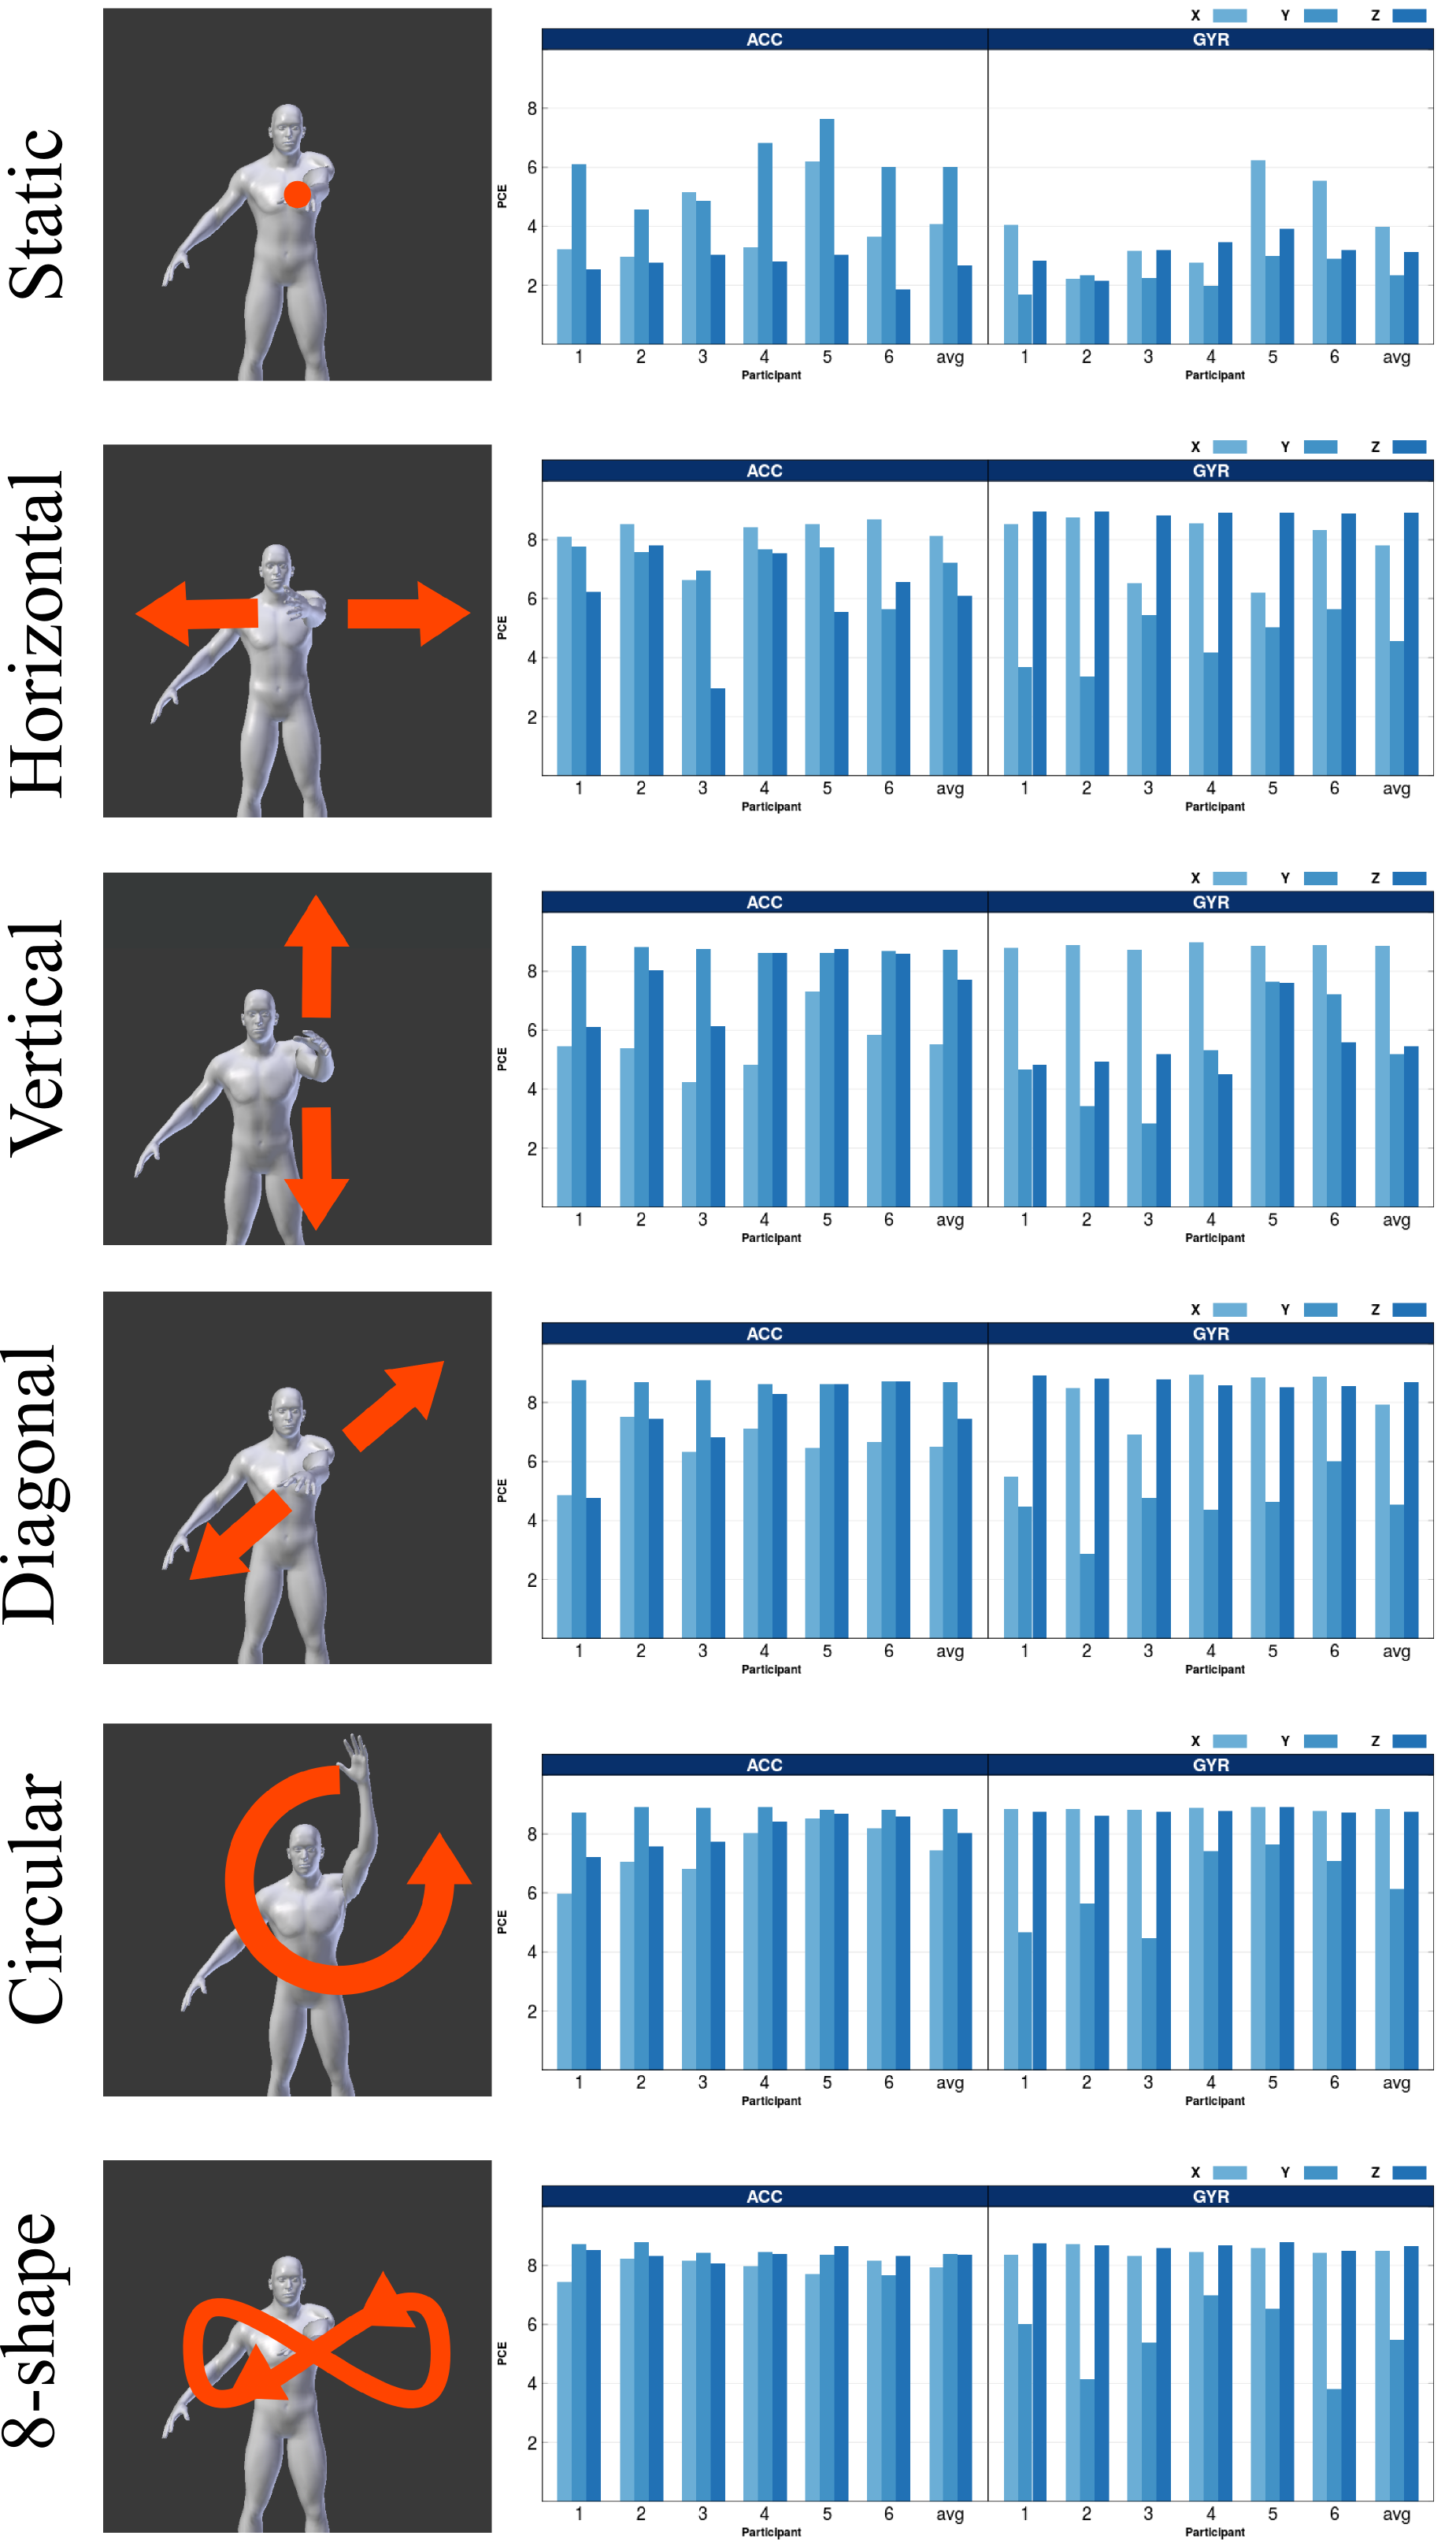
\includegraphics[width=1.0\linewidth]{movementsaucs04} 
\end{center}
}
  

\end{poster}

\end{document}
